\documentclass[preprint]{revtex4-1}
\usepackage{tikz}
\usepackage{pgfplots}
\usepackage{amsmath}
\usepackage{graphicx}
\usepackage{standalone}
\pgfplotsset{compat=newest, table/search path=figures}
\graphicspath{{./figures/}}

\begin{document}
\title{$\Sigma$RGO. Optimization of storage pricing} 

\author{VK}

\date{\today}

\begin{abstract}
    Present study is devoted to the basic analysis of the state size dynamics in
    $\Sigma$RGO system for different pricing policies with fair participants.
    The state is supposed to be used for data storage, and the price of storing
    the unit of data per unit time is supposed to depend on the state load.
    Continuous deterministic model of the dynamics leads to delayed differential
    equation.  Within the assumption of fixed storage duration, DDE takes the
    simple form, admitting analysis of the pricing for stability, and
    optimization of the miners' income. The results are discussed from the
    prospective of the optimal pricing (in terms of the ``soft'' state size
    restriction and high miners' rewards).
\end{abstract}

\maketitle

\section{Introduction}

The setup of the new currency admits the possibility of the information storage
in the state. Storing arbitrary data in the state is extremely expensive in
terms of device (PC, smartphone, server, or even toaster) usage. Hence, the
total state size must be restricted, and storage should provide some rewards to
the participants of the network, as it was proposed in [citation]. The idea is
to charge the participant storing the data in the network for the ``space-time''
consumption. The natural question arising in this kind of the situation is
``What should be the guiding principle of the price formation?''. The easiest
way is to set a rigid upper bound on the state size, set the price of storing,
say, 1 byte of information for 1 day. To make the setup more flexible, the
authors in [citation] proposed to adjust these parameters by referendum
conducted among the network participants. The rewards form the storage naturally
go to miners.

However, the question of the stability and sensitivity to initial conditions of
provided solution has stayed beyond the scope of discussion. Let me clarify the
last statement. At any given moment of time the system (state) is characterized
by the amount of the information stored and by the ``TTL'' (time to live) of
this information.  In other words, we have $N$ chunks of information, for every
chunk we have its size $L_i$, and the time it will stay in the system before
erasing $T_i$. The questions are: whether there is some stable configuration
such that in long run the system will stay approximately the same? If yes, is it
unique? And how strong does initial condition affects the long-run dynamics?

Preferable answers to this question would be yes-yes-``does not affect''. This
would mean that the state size does not oscillate, miners get stable salary, and
availability of storage is globally insensitive to local perturbations.

Another natural question arising is whether the rigid state size is necessary?
It is easy to imagine the situation where the formal possibility of exceeding
the state is still present, but hardly ever being used. For example, if one
wants to constrain the state size to 10MB, the possible solution is to set
normal price for submitting data to store if the state size after submission is
below 10MB, but some astronomical price for the luxury of storage above 10MB.
So, formally it will be possible, but in fact, hardly ever used, with every
usage bringing significant profit to miners. The generalization of this idea is
to form the explicit dependence of price on the state load (I will refer to it
as ``pricing curve''). The good pricing curve must provide at least one stable
equilibrium of the state size; the minimal dependence on initial conditions (if
possible), and high rewards for miners. The latter could serve as good
optimization parameter. Extreme cases are zero price -- huge data submission --
miners get nothing; and infinite price -- zero data submission -- miners get
nothing. As usual, the maximal outcome is between.  The pricing policies
described above are two particular cases of pricing curve (see
Fig.~\ref{fig:steps}).
\begin{figure}
    \hfill
    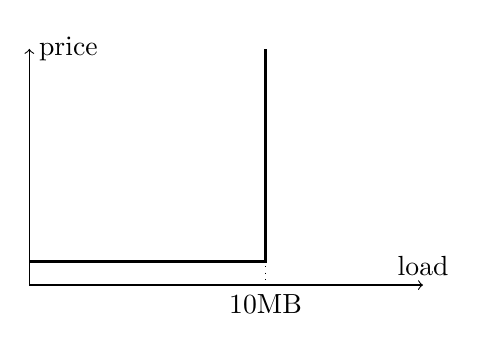
\begin{tikzpicture}
        \draw[->] (0,0) -- (0,3) node [right]{price};
        \draw[->] (0,0) -- (5,0) node [above]{load};
        \draw[very thick] (0,0.3) -- (3,0.3) -- (3,3);
        \draw[dotted] (3,1) -- (3,0) node[below]{$10$MB};
    \end{tikzpicture}
    \hfill
    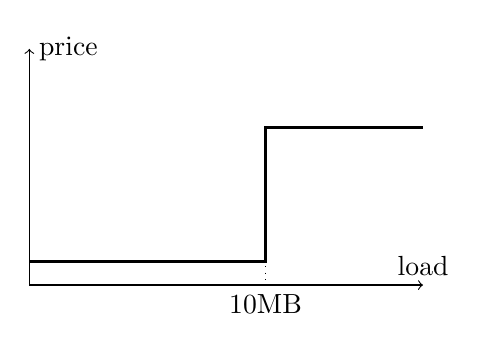
\begin{tikzpicture}
        \draw[->] (0,0) -- (0,3) node [right]{price};
        \draw[->] (0,0) -- (5,0) node [above]{load};
        \draw[very thick] (0,0.3) -- (3,0.3) -- (3,2) -- (5,2);
        \draw[dotted] (3,1) -- (3,0) node[below]{$10$MB};
    \end{tikzpicture}
    \hfill
    \caption{
        Examples of pricing curves: rigid state size [citation] (left) and
        overflow fees (right, see text). The value of $10$MB is taken
        arbitrarily.
        \label{fig:steps}
    }
\end{figure}

With the main questions posed above, the purpose of this work is basic analysis
of the storage dynamics in the situation of storage price depending on the
current state load. 

\section{Model}
For the primary analysis assume that participants act honestly: they submit
data if they need to do so and it is affordable; they do not in the opposite
case. For the sake of simplicity, suppose that the time of storage of data
block is fixed, and equal to $T$. In order to reduce the discrete stochastic
model to continuous deterministic one, assume that the number of participants
is large, and the typical size of the submitted data chunk is much less than
characteristic pricing curve variation scale. The amount of data submitted to
the state is changing continuously. At every given moment of time the users
submit the data at some rate (say, MB/s) $f$, which is defined by the current
price (participants submit more when cheap, and less when expensive). The
current price is fully determined by the current state load $x$. After time
interval $T$ data is erased from the state. The data is written into the state
at rate $f(x(t))$, and erased at rate $f(x(t-T))$. Under these assumptions,
the evolution of the state load is defined by the following equation:
\begin{equation}
    \frac{dx}{dt} = f(x(t))-f(x(t-T))\,.
    \label{eq:dde0}
\end{equation}
If one measures time in the data block TTL $T$, the equation takes the form
\begin{equation}
    \dot{x} = f(x(t))-f(x(t-1))\,.
    \label{eq:dde1}
\end{equation}
The equations of this type are called delay differential equations (DDE), and have
been studied widely for the vast amount of control problems.

Now few words about the function $f$, and how to convert it to the miner's
income. What participants know is the pricing curve $p(x)$. For every value $P$
of this function there is amount of people $N(P)$ who want to submit data and
can afford it at time interval $T$. The function $N(P)$ is non-increasing, and
going to zero for sufficiently large $P$ (every participant has maximal price he
is ready to pay, and will also try to submit something if current price is
lower; for sufficiently large price no one is ready to pay). In these notations
$f(x)=N(p(x))$ (see inset on Fig.~\ref{fig:rewards}), and the profit rate which
miners get from current submissions is $y(t) = p(x(t))f(x(t))$.

\section{Stability}

Assume that at some point the state size achieved constant value $x^*$. As one
can see from the Eq.~\eqref{eq:dde1}, any value of the sate size can be an
equilibrium. That is, the rate of writing data is exactly equal to the rate of
erasing. In order to figure out the stability of the equilibrium state, one can
linearize Eq.~\eqref{eq:dde1}, and obtain the following equation for the
perturbed solution $x=x^*+\delta x$:
\begin{equation}
    \delta\dot{x}(t) = f'(x^*)[\delta x(t)-\delta x(t-1)]\,.
    \label{eq:perturb}
\end{equation}
After the substitution $\delta x(t) = Ae^{\lambda t}$, one obtains
\begin{equation}
    \lambda = f'(x^*)(1-e^{-\lambda})\,.
    \label{eq:eigen}
\end{equation}
If Eq.~\eqref{eq:eigen} has the solution $\lambda$ such that $Re(\lambda)>0$,
the equilibrium is unstable. If $f'(x^*)>1$, there is one obvious real positive
root, so the equilibrium is unstable. Taking imaginary part of the equation, one
can see the absence of another values $\lambda$ with positive real part.
\begin{figure}
    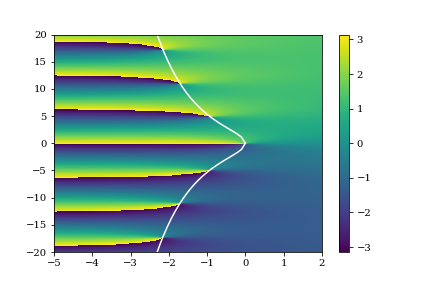
\includegraphics{eigenvals}
    \caption{
        \label{fig:eigen}
        Spectrum of the model.
    }
\end{figure}

\subsection{Rigid size restriction}

\subsection{Soft size restriction}

\begin{figure}
    \includestandalone[width=\textwidth]{figures/dynamics}
    \caption{
        \label{fig:dynamics} Dynamics of the state size for various initial
        rates. The numbers above the curves are the miners reward rates with
        respect to maximal possible stationary rewards.
    }
\end{figure}
\section{Rewards optimization}

Recall that the rewards rate obtained by the miners for stable state size at
price $p$ is given by $y=pN(p)$. Example is provided at Fig.~\ref{fig:rewards}
First, it provides a possible method of measuring explicit form of the function
$N(p)$ in the model: one has to set up the price, and observe the static
rewards. Second, one may wonder about the price $p^*$, optimal for the miners in
terms of rewards. Obviously, it satisfies $N(p^*)+p^*N'(p^*)=0$, where prime is
derivative with respect to price. As usual, the optimal price here does not
depend on the pricing policy, but rather the implicit property of the network.
Having the price varying freely can be considered beneficial both for miners and
for network as a whole, since it allows the first ones to optimise signing
strategy, and with this given the state size is automatically adjusted to the relatively
predictable level $p^{-1}(p^*)$.

\begin{figure}
    \includestandalone[width=\textwidth]{figures/rewards}
    \caption{
        \label{fig:rewards} Rewards curve.
    }
\end{figure}

\section{Sensitivity with respect to initial conditions}


\section{Example}
From what was said above, the conclusion is that two values are particularly
important for the model: maximal state size, and optimal price. In order to
preserve the limitation on the stored amount of data, one can let the storage price go to infinity
faster than $1/x$ moving closer to the limiting size. On the other side, there
may be some intermediate ``preferred'' size of the state $x_d$. This, in turn,
can be matched to the optimal price. One may also wish to introduce the lower
bound on the storage price $p_{min}$. Taking these values it is easy to
construct the function $p(x)$ with the desired properties. As an example,
\begin{equation}
    p(x) = p_{min}+(p^*-p_{min})\frac{x}{x_d}\frac{x_{max}-x_d}{x_{max}-x}\,,
    \label{eq:sample_price}
\end{equation}
Another question is how one should deal with the chunks of data comparable to
the state size. The logical way is to treat $p(x)$ as the differential property
(which it actually is). So if the current state size is $x_0$, and the
participant is willing to submit the data block of size $L$ for unit time, he is
charged by the amount of $\int_{x_0}^{x_0+L}p(x)\,dx$. For the sample pricing
curve it is
\begin{equation}
    P = L\left(p^*-\eta \Delta p \right)
    -
    \eta(\eta-1)\Delta p\, x_d
    \log\left(1-\frac{L}{x_{max}-x_0}\right)\,,
    \label{eq:sample_chunk}
\end{equation}
where $\eta=x_{max}/x_d$,$\Delta p=p^*-p_{min}$. Note that the logarithmic
divergence guards the upper size limit.

\section{Discussion}
The idea of soft restriction of the state size, and having the floating storage
price is flexible an appealing both in the context of fast reaction on the
environment change, and making mining rewarding. The strong side of the scheme
is the possibility of automatic adjustment during the transactions. The
fluctuations in the storage demand on the intermediate scale (more than typical
storage period, but less than extending the storage capability and hardware) do
not require any changes in the network rules, and the optimal (in terms of
mining) regime can always be achieved.

However few things could require more detailed investigation. First, the model
used in the study is very simplistic. It does not incorporate stochastic effects
by itself, neither it assumes any variation in the storage time. This allowed
studying the simple differential equation with transparent meaning. But as a
backside, the model has infinite memory, which was discussed above. In realistic
situation the memory can be long, but it is unlikely to stay infinite. The
expected source of that is the stochastic effects. Second, as it was mentioned,
potentially any state size can be an equilibrium one. This is inevitable for the
described model, and is a consequence of the balance between storing and erasing
no matter at which rate. From the side of DDE, it can be viewed as lack of
``dissipation''. It may also seem beneficial to have more stable system, where
the equilibrium state is more predictable. But this would most likely imply more
sophisticated price formation policy. Finally, the technical side of the
transaction organisation and sharing charges is also beyond the discussion, as
well, as different types of attacks and unfaithful cooperation.

As these obstacles are certainly very important for the technical realisation,
the general setup is believed to stay unaffected by the first two, which indeed
makes it a good candidate for the stable, flexible and relatively predictable
chain.

\bibliography{sources}
\end{document}
